\section{Pausing environment}
\label{sec:pause}

We first formally define the simplified syntax of \Hazel shown in Figure \ref{fig:syntax} \cite{HazelLive}. The symbol $\ehole$ represents the empty hole used to indicate the place that need to fill in the incomplete program. And for the expression that doesn't have clear meaning, we use $\llparenthesiscolor e \rrparenthesiscolor$ to indicate that it doesn't have semantic meanings. We only consider binary sums so for $\hinj{i}{e}$,  $i \in \{L, R\}$.

\begin{figure}[htbp]
    \vspace{-3px} 
  $\arraycolsep=4pt\begin{array}{lll}
  HTyp~~ \tau & ::= &
    \tnum  ~\vert~
    \tarr{\tau}{\tau} ~\vert~
    (\tau + \tau) ~\vert~
    \ehole^A
    \\
  HExp~~ e & ::= &
    x ~\vert~
    \lamfunc{x}{e} ~\vert~
    \lamfunc{x:\tau}{e} ~\vert~
    e(e) ~\vert~
    \underlinenum{n} ~\vert~
    (e+e) ~\vert~
    e: \tau ~\vert~
    \hinj{i}{e} ~\vert~
    \hcase{e}{x}{e}{y}{e}~\vert~
    \ehole  ~\vert~
    \notehole{e} 
  \end{array}$
  \hrule
  \caption{Syntax of H-types, H-expressions}
    \label{fig:syntax}
    \vspace{-5px}
\end{figure}

\begin{figure}[htbp]
    \vspace{-3px} 
    \fbox{ $\isPaused{e} $}~~\text{$e$ is paused}\hfill
    \begin{subequations}\label{eqns:paused}
    \begin{mathpar}
        \hfill
        \inferrule[PCaseHole]{
            }{
              \isPaused{\hap{\lamfunc{z}{\hcase{z}{x}{e_1}{y}{e_2}}}{\ehole}}
            }
        \hfill
        \inferrule[PCase]{ \isPaused{e_0}
            }{
              \isPaused{\hcase{e_0}{x}{e_1}{y}{e_2}}
            }
        \hfill\hfill
    \end{mathpar}
    \begin{mathpar}
        \hfill
        \inferrule[PAp1]{ \isPaused{e_1}
            }{
              \isPaused{\hap{e_1}{e_2}}
            }
        \hfill
        \inferrule[PAp2]{ \isPaused{e_2}
            }{
              \isPaused{\hap{e_1}{e_2}}
            }
        \hfill
        \hfill
    \end{mathpar}
    \begin{mathpar}
        \hfill
        \inferrule[PAdd1]{ \isPaused{e_1}
            }{
              \isPaused{e_1 + e_2}
            }
        \hfill
        \inferrule[PAdd2]{ \isPaused{e_2}
            }{
              \isPaused{e_1 + e_2}
            }
        \hfill
        \inferrule[PHole]{ \isPaused{e}
            }{
              \isPaused{\hhole{e}}
            }
        \hfill
        \hfill
    \end{mathpar}
    
    \end{subequations}
    \caption{Paused forms}
    \label{fig:paused_forms}
    \vspace{-5px}
\end{figure}

Normally, we have judgement like $\mathtt{final}$, $\mathtt{boxedvalue}$ for a program. Furthermore, since \Hazel contains incomplete programs, there exists some indeterminate programs which induces a judgement called $\mathtt{indet}$ \cite{HazelnutPOPL}. Pausing judgement is noted as $\mathtt{paused}$. For example, when $\ehole$ appears at case expression so that the match algorithm gives indeterminate result, it will be a paused expression so that the stepper can stop immediately. Figure \ref{fig:pause} gives a expression as example. It defines a function func. But we don't provide any argument for it. The evaluator expand the case expression directly. However, the result in bottom shows an example that when augment is only a hole, the stepper will not evaluate but stop with yellow box indicating it is steppable but paused.

% \begin{figure}[htbp]
%     \centering
%     \begin{subfigure}[b]{0.4\textwidth}
%         \centering
%         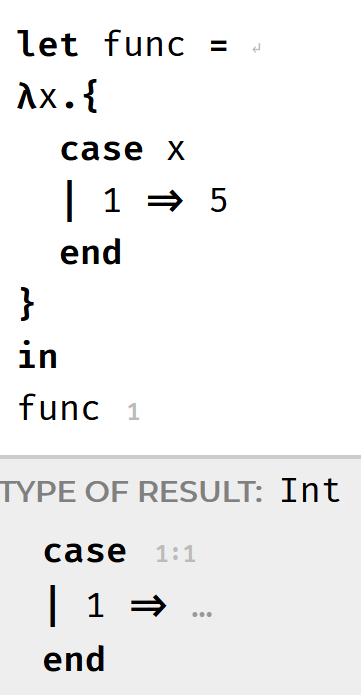
\includegraphics[width=0.4\textwidth]{img/case1.png}
%         \caption{}
%         \label{fig:pause1}
%     \end{subfigure}
%     \begin{subfigure}[b]{0.4\textwidth}
%         \centering
%         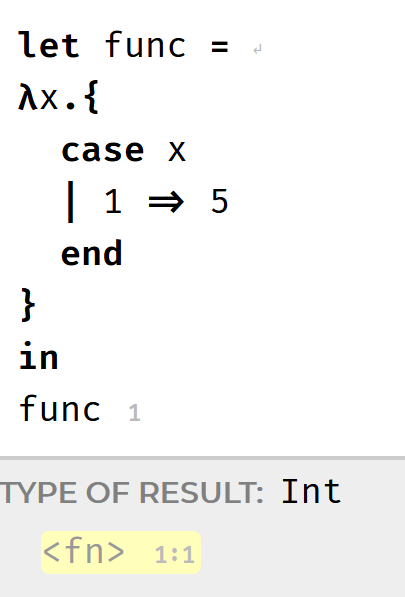
\includegraphics[width=0.5\textwidth]{img/case2.png}
%         \caption{}
%         \label{fig:pause2}
%     \end{subfigure}
%     \caption{Example of stepper with paused environment}
% \end{figure}